\documentclass[11pt]{article}
\usepackage[hmargin=1in,vmargin=1in]{geometry}
\usepackage[document]{ragged2e}
\usepackage{xcolor}
\usepackage{amsmath,amssymb,amsfonts,url,sectsty,framed,tcolorbox,framed}
\usepackage{tikz}
\usepackage{nicematrix}
\newcommand{\pf}{{\bf Proof: }}
\newtheorem{theorem}{Theorem}
\newtheorem{lemma}{Lemma}
\newtheorem{proposition}{Proposition}
\newtheorem{definition}{Definition}
\newtheorem{remark}{Remark}
\newcommand{\qed}{\hfill \rule{2mm}{2mm}}


\begin{document}
%%%%%%%%%%%%%%%%%%%%%%%%%%%%%%%%%%%%%%%%%%%%%%%%%%%%%%%%%%%%%%%%%%%%%
\noindent
\rule{\textwidth}{1pt}
\begin{center}
{\bf [CS304] Introduction to Cryptography and Network Security}
\end{center}
Course Instructor: Dr. Dibyendu Roy \hfill Winter 2022-2023\\
Scribed by: Chitranshi Srivastava (202051055) \hfill Lecture 8 and 9 (Week \#5)
\\
\rule{\textwidth}{1pt}
%%%%%%%%%%%%%%%%%%%%%%%%%%%%%%%%%%%%%%%%%%%%%%%%%%%%%%%%%%%
%write here
In the previous week, we started mathematical recall about groups, abelian groups and finite groups before moving ahead to AES.
\section{Mathematics Recall}

\subsection{Generators and Cyclic Group}
Consider a group $(G, *)$. Let $\alpha \in G$. The identity element $\alpha^0$ belongs to G. Therefore,
\begin{center}
    $\alpha^0 * \alpha = \alpha^1$\\
    \vspace{1mm}
    $\alpha^1 * \alpha = \alpha^2$\\
    \vspace{1mm}
    $\alpha^2 * \alpha = \alpha^3$\\
\end{center}
\textbf{Note: }The $*$ here is not multiplication, it is a binary operation not necessarily multiplication. $\alpha^1, \alpha^2, \alpha^3$ and so on, are just notation of using the binary operation $*$ on same element. \\
\vspace{5mm}
Since, G is closed under $*$, any two elements belonging to G, will give the result in G on performing the binary operation $*$. Since $\alpha^0 \in G$ and $\alpha \in G$, therefore $\alpha^1 \in G$. Now, since $\alpha^1 \in G$, therefore $\alpha^2 \in G$, and so on. That means,
\begin{center}
    $\alpha^0, \alpha^1, \alpha^2, ... \in G$
\end{center}
The set $\alpha^0, \alpha^1, \alpha^2, ...$ is denoted by $\langle \alpha \rangle$. Also, $\langle \alpha \rangle \subseteq G$. $\alpha$ is called the generator of $(G, *)$ iff:
\begin{center}
    for any $b \in G$ $\exists$ $i \geq 0$ such that $b = \alpha^i$ and hence $G \subseteq \langle \alpha \rangle $. 
\end{center}
\textbf{We can conclude that $(G,*) = \langle \alpha \rangle $}\\
A group is called a cyclic group if there is an element $\alpha \in G$, such that for every $b \in G$, there is an integer $i$ with $b = \alpha^i$. In simple words, every element in G can be expressed as some exponent of $\alpha$, then $\alpha$ is the generator of G.
\vspace{3mm}
\subsubsection{Order of an element}
Consider (G,*) and $|G|$ : finite. Let a$\in$G.\\
We already know that $a^0$ is identity. Now, the order of an element is the least positive integer m such that $a^m = e$. 
\begin{center}
    o(a) = m such that $a^m$ = e
\end{center}
Since $a^m = e$, so $a^{m+1}=a$, $a^{m+2}=a^2$ and so on. So we define a set H such as:
\begin{center}
    H = $\{a^0, a^1, a^2.....a^{m-1}\}$
\end{center}
We understand that
\begin{itemize}
    \item $H \subseteq G$
    \item H is a group under *
\end{itemize}
\subsection{Lagrange's Theorem}
If G is a finite group and H is a subgroup of G, them $|H|$ divides $|G|$.
\vspace{3mm}
G is a finite group and a$\in$G. We know that 
\begin{center}
    H = $\{a^0, a^1, a^2.....a^{o(a)-1}\}$
\end{center}
and H is a subgroup of G. $|H|=a(a)$.
\\So, using Lagrange's theorem, we can conclude that
\begin{center}
    $|H|$ $|$ $|G|$ $\Rightarrow$ o(a) $|$ $|G|$
\end{center}
\subsection{Some Results}
\begin{itemize}
    \item If the order of a$\in$G is t, then
    \begin{center}
        o($a^k)$ = \(\frac{t}{gcd(t,k)}\)
    \end{center}
    \item If gcd(t,k) = 1, then\\
    \begin{center}
        o($a^k) = t = o(a)$\\
        $\Rightarrow |\langle a^{k} \rangle| = |\langle a \rangle|$
    \end{center}
    Let x $\in \langle a^k \rangle$, then x = $(a^K)^i$ = $a^{ki}$\\Now ki is also some integer so $a^{ki} \in \langle a \rangle$.\\So, $\langle a^k \rangle \subseteq \langle a \rangle$. But the number of elements in both the sets is same. So, $\langle a^k \rangle = \langle a \rangle$.\\ Hence, $a^k$ is also the generator of  $\langle a \rangle$.\\
\end{itemize}
\vspace{3mm}
\textbf{Example:}\\
$Z^*_{19}$ = $\{ x | gcd(x,19)=1, 1 \leq x \leq 18 \}$, where\\
$*_{19}$ : multiplication modulo 19 and\\
x $*_{19} $ y = (x $\dot 
 $ y) mod 19\\
Find the generators of ($Z^*_{19},*_{19}).$\\
\textbf{Solution:}\\
x$\in Z^*_{19}$\\
S = $\{ x^0, x^1 ......\}$\\
Now let us check.\\
$\langle 2 \rangle$ = $\{ 1, 2, 4, 8, 16, 7, 14, 9, 18, 17, 15, 11, 3, 6, 12, 5, 10\}$ = $Z^*_{19}$\\
So, o(2) = 18.\\
Let us see for $2^2$: gcd(19,2) $\neq$ 1, so $2^2$ is not a generator.\\
gcd(18,5) = 1, so $2^5$ is also a generator and so on.

\subsection{Ring}
A ring (R, $+_R, \times_R)$ consists of one set R with two binary operations arbitrarily denoted by $+_R$(addition) and $ {\times}_R$(multiplication) on R satisfying the following properties
\begin{itemize}
    \item $(R, +_R)$ is an abelian(commutative) group with the identity element $0_R$
    \item The operation $\times_R$ is associative,i.e,
    \begin{center}
        $a \times_R (b \times_R c)$ = $(a \times_R b) \times_R c$
    \end{center}
    \item There is a multiplicative identity denoted by $1_R$ with $1_R \neq 0_R$ such that 
    \begin{center}
        $1_R \times_R a = a \times_R 1_R = a$ $ \forall a\in R$
    \end{center}
    \item The operation $\times_R$ is distributive over $+_R$, i.e,
    \begin{center}
        $(b+_Rc)\times_R a = (b\times_Ra) +_R (c\times_Ra)$ and\\
        $a\times_R(b+_Rc) = (a\times_Rb) +_R (a\times_Rc)$ and\\
    \end{center}
\end{itemize}
\textbf{Example:}\\
(R, $+_R, \times_R$ ) : check it is a ring or not.\\
\textbf{Solution:}\\
$(R, +_R)$ is a commutative group with identity element 0 and -x as inverse. Real number 1 is identity and multiplication is associative and distributive hence it is a ring.

\subsubsection{Commutative Ring}
If the second operation is commutative, i.e, $a\times_Rb = b\times_Ra$, then it is commutative ring.

Both (R, $+_R, \times_R ) and (Z, +, \cdot$ ) are commutative rings.\\
\vspace{3mm}
\textbf{\underline{Note}:} Under the second operation, it does not necessarily be a group. It is not guaranteed that a multiplicative inverse will always be present. \\
If such elements are present that have multiplicative inverse(like 1 in case of Z), we call those elements as unit elements or invertible elements of the ring such that
\begin{center}
    $a\times_Rb = 1_R$
\end{center}

\textbf{Example:}\\
$(Z_n, +_n, *_n)$ is a ring?\\
\textbf{Solution:}\\
First operatiom forms an abelian group over $Z_n$. For $*_n$, 0 is the identity and it is both associative and distributive. Hence it is a ring. For all x in $Z_n$, if gcd(x, n)=1, then x has multiplicative inverse and it is unit element.

\textbf{Note:} The set of units in a ring R form a group under multiplication operation. This is known as group of units of R.

\subsection{Field}
A field is a non-empty set F together with two binary operation +(addition) and *(multiplication) fow which the following properties are satisfied
\begin{itemize}
    \item (F, +) is an abelian group
    \item If $0_F$ denotes the additive identity element of (F,+) then (F $\backslash \{0_F\}, *) $ is a commutative/abelian group.
    \item $\forall$ a,b,c $\in$ F, we have,
    \begin{center}
        a*(b+c) = (a*b) + (a*c)
    \end{center}
\end{itemize}
\vspace{5mm}
\textbf{Example:}\\
$(Z_P, +_P, *_P)$ is a Field ? Here, P is a prime number.\\
\textbf{Solution:}\\
Under, $+_P$ it is always an abelian group with 0 as identity element. Under $*_P$ is always associative and distributive. For all $Z_P - 0$, there is always an inverse under $*_P$ because since P is prime, gcd(x, P) = 1 always. So, $*_P$ forms a commutative group on $Z_P-0$.Hence, it is a Field.\\
\vspace{3mm}
\textbf{Note:}\\
\begin{itemize}
    \item $(Z, +, \cdot)$ is not a field because inverse does not exist
    \item $(Q, +, \cdot)$\\
    (Q, +) : abelian group\\
    0 : additive identity\\
    1 : multiplicative identity\\
    $(Q \backslash \{0\}, \cdot$ forms an abelian group.\\
    Hence, it is a field.
\end{itemize}
\textbf{Example:} Is $(\mathbb{F}_p, +_p, *_p)$ a field, where p is a prime number?\\
\textbf{Solution:} We know that $(\mathbb{F}_p, +_p)$ an abelian group with identity element 0. Now, the set $\mathbb{F}_p - \{0\}$ has existing multiplicative inverse iff gcd(x, p) = 1 for each $x \in \mathbb{F}_p - \{0\}$. Since, p is prime, gcd(x, p) = 1 for all possible integers that $x$ can take. Hence, $(\mathbb{F}_p, +_p, *_p)$ is a field.\\


%Lecture 9 

\section{Field Extension}
Suppose $K_2$ is a field with addition(+) and multiplication(*). \\
Suppose $K_1 \subseqeq K_2$ is closed under both these operations such that $K_1$ itself is a field with the restriction of + and * to the set $K_1$. Then $K_1$ is called a subfield of $K_2$ and $K_2$ is called a field extension of $K_1$.

\section{Polynomial Ring}
Let $(F, +, *)$ be a field and the set of polynomials of any degree $F[x]$ be:
\begin{center}
    $F[x] = \{a_0 + a_1\cdot x + a_2 \cdot x^2 +.... | a_i \in F\}$
\end{center}
$F[x]$ is set of all polynomials in $x$ with coefficients belonging to set F of the given field. The set of polynomials along with the binary operations of the field forms a ring and this ring is known as polynomial ring.

\begin{center}
    $(F[x], +, *) \rightarrow$ Polynomial Ring\\
    \vspace{1mm}
    $P_1(x) \in F[x] = a_0 + a_1 \cdot x +....+ a_n \cdot x^n$\\
    \vspace{1mm}
    $P_2(x) \in F[x] = b_0 + b_1 \cdot x +....+ b_n \cdot x^n$\\
\end{center}
If we want to add the two polynomials,
\begin{center}
    $P_1(x) + P_2(x) = (a_0 + a_1 \cdot x +....+ a_n \cdot x^n) + (b_0 + b_1 \cdot x +....+ b_n \cdot x^n)$\\
    \vspace{1mm}
    $P_1(x) + P_2(x) = (a_0 + b_0) + (a_1 + b_1) \cdot x +.....+ (a_n + b_n) \cdot x^n$
\end{center}
The coefficients $a_i, b_i$ belong to set F and the addition operation is the field addition of the field $(F, +, *)$. Since $(F, +, *)$ is a field, therefore, $(F, +)$ is an abelian group and addition on elements of F is closed. Therefore, $P_1(x) + P_2(x)$ is closed under addition because for any $i$, $(a_i + b_i) \in F$. Also, addition of polynomials is just coefficient-wise, hence, addition of polynomials will be associative because of field properties of coefficients. Similarly, the additive identity of field will be the additive identity of the polynomial in $F[x]$. Now, let's look at additive inverse of $P(x)$.
\begin{center}
    $P(x) = a_0 + a_1 \cdot x +.....+ a_n \cdot x^n$\\
    $P(-x) = -a_0 + (-a_1) \cdot x +.....+ (-a_n) \cdot x^n$\\
\end{center}
Clearly, $P(-x)$ is additive inverse of $P(x)$. Here, the negative sign does not mean the standard negation. It implies the additive inverse of $a_i$ in the field F. Also, 
\begin{center}
    $P_1(x) + P_2(x) = P_2(x) + P_1(x)$
\end{center}
Therefore, under addition the polynomial set $F[x]$ is an abelian group. Now, let's look at the multiplication operation of the two polynomials:
\begin{center}
    $P_1(x) * P_2(x) = (a_0 + a_1 \cdot x +....+ a_n \cdot x^n) * (b_0 + b_1 \cdot x +....+ b_n \cdot x^n)$\\
    \vspace{1mm}
    $P_1(x) * P_2(x) = (a_0 * b_0) + (a_0 * b_1 + b_0 * a_1) \cdot x +.....+ (a_n * b_n)\cdot x^n$
\end{center}
The multiplication operation is field multiplication operation and hence is associative, distributive. Also, the multiplicative identity also exists for the polynomials in $F[x]$. Hence, $(F[x], +, *)$ is a polynomial ring.

Let us define a polynomial ring formally. A set of polynomials $F[x]$ along with the operation of addition(+) and multiplication(*) is called a ring if:
\begin{enumerate}
    \item $(F[x], +)$ is an abelian group.
    \item * is associative over $F[x]$.
    \item An identity element over multiplication exists.
    \item * is distributive over +.
\end{enumerate}

\textbf{Example:} Consider the set $\mathbb{F} = \{0, 1\}$ and the field $(\mathbb{F}, +_2, *_2)$. Therefore, the polynomial set $\mathbb{F}_2[x]$ is:
\begin{center} 
    $\mathbb{F}_2[x] = \{a_0 + a_1 \cdot x + .... | a_i \in \mathbb{F}\}$
\end{center}
Let us just take two polynomials from this set:
\begin{center}
    $p(x) = x + 1$\\
    \vspace{1mm}
    $q(x) = x^2 + x + 1$\\
    \vspace{1mm}
    $p(x) +_2 q(x) = (x + 1) +_2 (x^2 + x + 1) = x^2 + (1 +_2 1) \cdot x + (1 +_2 1) = x^2$ \\
    \vspace{1mm}
    $p(x) *_2 q(x) = (x + 1) *_2 (x^2 + x + 1)$\\
    \vspace{1mm}
    $p(x) *_2 q(x) = (x^3 + x^2 + x) + (x^2 + x + 1) = x^3 + (1 +_2 1) \cdot x^2 + (1 +_2 1) \cdot x + 1$\\
    \vspace{1mm}
    $p(x) *_2 q(x) = x^3 + 1$
\end{center}

\section{Irreducible Polynomial}
A polynomial $P(x) \in F[x]$ of degree $n \geq 1$ is called irreducible if it cannot be written in the form of $P_1(x) * P_2(x)$ with $P_1(x), P_2(x) \in F[x]$ and degree of $P_1(x), P_2(x)$ must be greater than or equal to 1. It means that $P(x)$ is irreducible if it can not be factorised.\\
\newline
\textbf{Example:} $x^2 + 1 \in \mathbb{F}_2[x]$.\\
\textbf{Solution:} $(x + 1) * (x + 1) = x^2 + (1 + 1) \cdot x + 1 = x^2 + 1$. Therefore, $(x^2 + 1) =  (x + 1) * (x + 1)$ in $\mathbb{F}_2[x]$. Hence, $(x^2 + 1)$ is reducible in $\mathbb{F}_2[x]$. Note that it is not possible to factor $x^2 + 1$ in $\mathbb{R}[x]$, where $\mathbb{R}$ is set of real numbers.\\

\subsection{Ideal Generated by P(x)}
It is a set denoted by I which contains the polynomials given as:
\begin{center}
    $I = \langle P(x) \rangle = \{q(x) \cdot P(x) | q(x) \in F[x]\}$
\end{center}

Consider the set denoted by $F[x]/\langle P(x)  \rangle$ whose each element is formed by taking an element from $F[x]$ and then dividing it by $P(x)$. That is,
\begin{center}
    $q(x) \in F[x] = d(x) * P(x) + r(x)$\\
    \vspace{1mm}
    $r(x) \in F[x]/\langle P(x)  \rangle$
\end{center}
The remainder obtained belongs to the set $F[x]/\langle P(x)\rangle$. Now, if P(x) is irreducible polynomial, then $(F[x]/\langle P(x) \rangle, +, *)$ becomes a field. Here, the addition and multiplication operation are under modulo P(x). The degree of r(x) is always lesser than degree of P(x).\\

\textbf{Example:} $x^2 + x + 1 \in F_2[x], F_2 = \{0, 1\}$. $P(x) = x^2 + x + 1$ is irreducible.\\

Consider the set $F_2[x]/\langle x^2 + x + 1\rangle$:
\begin{center}
    $q(x) = d(x) \cdot P(x) + r(x)$\\
    $deg(r(x)) < 2$\\
    $r(x) = \{0, 1, x, x + 1\}$
\end{center}

If P(x) is a n degree polynomial under modulo 2, then there will be $2^n$ polynomials in r(x), that is, $F_2[x]/\langle x^2 + x + 1\rangle$.

Consider now for example a polynomial $X^2 + 1 \in F_2[x]$. Let's find the remainder on dividing it by P(x). For $F_2$, the remainder can be found in an easy way. It can be done by replacing $x^2$ in dividend with the lesser degree part of divisor, that is, $(x + 1)$. Therefore, 
\begin{center}
    $x^2 + 1 = q(x) * (x^2 + x + 1) + r(x)$\\
    $r(x) = x + 1 + 1 = x$
\end{center}

Let's take another example, say, $x^3 + 1$:
\begin{center}
    $x^3 + 1 = q(x) * (x^2 + x + 1) + r(x)$\\
    $r(x) = x \cdot x^2 + 1 = x \cdot (x + 1) + 1$\\
    $r(x) = x^2 + x + 1 = x + 1 + x + 1 = 0$
\end{center}
We saw that the remainder came out to be 0 and x. We can take other examples where the remainder will come out to be the remaining two polynomials, that are, 1 and $(x + 1)$.

\section{Primitive Polynomial}
Consider the set $F_2[x]/\langle x^2 + x + 1\rangle$. We have discussed that if the P(x) is irreducible then $(F[x]/\langle P(x) \rangle, +, *)$ becomes a field. Now, let's say if $\alpha$ is a root of $x^2 + x + 1 = 0$, that is,
\begin{center}
    $\alpha^2 + \alpha + 1 = 0$\\
    $\alpha^2 = -\alpha + (-1) = \alpha + 1$
\end{center}
If $\alpha$ can generate all the possible polynomials in $F_2[x]/\langle x^2 + x + 1\rangle$, then $x^2 + x + 1$ is known as primitive polynomial. Now, let's see:
\begin{center}
    $\langle \alpha \rangle = \{0, 1 = \alpha^0, \alpha, \alpha + 1 = \alpha^2\}$\\
    $O(\alpha) = 2$
\end{center}
Hence, $x^2 + x + 1$ is a Primitive Polynomial.\\

\textbf{Example:} $\mathbb{F}_2[x]/\langle x^3 + x + 1 \rangle$\\
\textbf{Solution:} The maximum number of polynomials that can be generated:
\begin{center}
    $\{0, 1, x, x + 1, x^2, x^2 + 1, x^2 + x, x^2 + x + 1\}$
\end{center}
Let's check if root of $x^3 + x + 1 = 0$ is a generator or not.
\begin{center}
    $\alpha^3 + \alpha + 1 = 0 \implies \alpha^3 = \alpha + 1$\\
    \vspace{1mm}
    $\langle \alpha \rangle = \{0, 1 = \alpha^0, \alpha, \alpha^2, \alpha + 1 = \alpha^3, \alpha^2 + \alpha = \alpha^4, \alpha^2 + \alpha + 1 = \alpha^5, \alpha^2 + 1 = \alpha^6\}$
\end{center}
Since, we are able to generate all the polynomials, therefore $x^3 + x + 1$ is a primitive polynomial. Note that there may exists a polynomial that is not a primitive polynomial but is still a field. That means, we will be able to find multiplicative inverse. Let us consider for the polynomial $x$. Instead of 1/x, we have a polynomial $x^2 + 1$, which will give 1 as result on multiplication.
\begin{center}
    $x * (x^2 + 1) = x^3 + x = x + 1 + x = 1$
\end{center}
Similarly, for $x^2$ the multiplicative inverse is $x^2 + x + 1$.
\begin{center}
    $x^2 * (x^2 + x + 1) = x^4 + x^3 + x^2 = x * (x + 1) + (x + 1) + x^2$\\
    $x^2 * (x^2 + x + 1) = x^2 + x + x + 1 + x^2 = 1$
\end{center}

\section{Advanced Encryption Standard}
When the design of DES was made public, it was immediately broken. Thereafter, NIST called for a competition named Advanced Encryption Standard. A lot of cryptographers around the world submitted their designs along with the implementation. One of the submission in the competition was $\emph{Rijndael}$. It was developed by two Belgian cryptographers, Joan Daemen and Vincent Rijmen. In the proposal, it was mentioned that the winner will be renamed as Advanced Encryption Standard. AES is unbreakable till date.\\

Advanced encryption Standard is an iterated block cipher and is based on Substitution Permutation Network(SPN). There are three different variants of AES:
\begin{enumerate}
    \item AES-128 (Block Size 128-bit, Number of Rounds = 10, Secret Key Size 128-bit)
    \item AES-192 (Block Size 128-bit, Number of Rounds = 12, Secret Key Size 192-bit)
    \item AES-256 (Block Size 128-bit, Number of Rounds = 14, Secret Key Size 256-bit)
\end{enumerate}

\subsection{AES 128}

\begin{center}
    \tikzset{every picture/.style={line width=0.75pt}}
    
    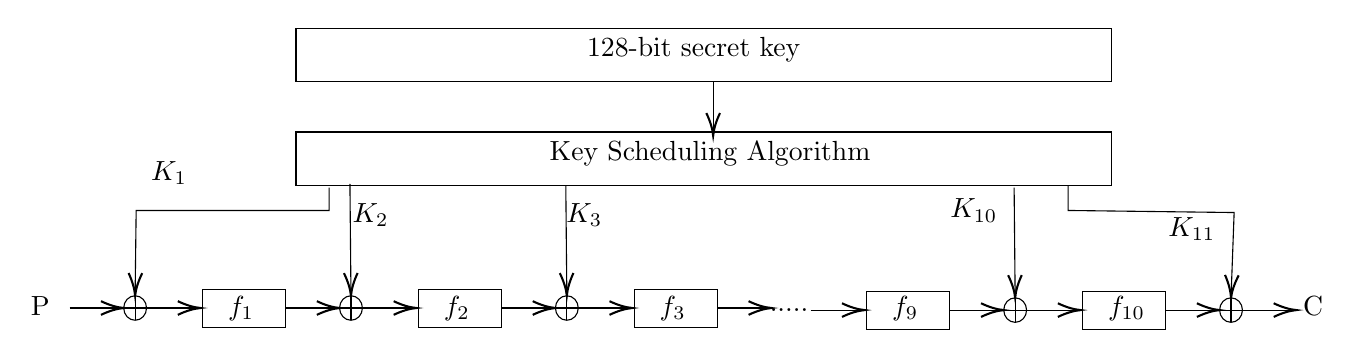
\begin{tikzpicture}[x=0.75pt,y=0.75pt,yscale=-1,xscale=1]
        \draw   (146,38) -- (539,38) -- (539,63.8) -- (146,63.8) -- cycle ;
        \draw    (347,63.8) -- (347,87.8) ;
        \draw [shift={(347,89.8)}, rotate = 270] [color={rgb, 255:red, 0; green, 0; blue, 0 }  ][line width=0.75]    (10.93,-3.29) .. controls (6.95,-1.4) and (3.31,-0.3) .. (0,0) .. controls (3.31,0.3) and (6.95,1.4) .. (10.93,3.29)   ; 
        \draw   (146,88) -- (539,88) -- (539,113.8) -- (146,113.8) -- cycle ;
        \draw    (37,172.8) -- (61,172.8) ;
        \draw [shift={(63,172.8)}, rotate = 180] [color={rgb, 255:red, 0; green, 0; blue, 0 }  ][line width=0.75]    (10.93,-3.29) .. controls (6.95,-1.4) and (3.31,-0.3) .. (0,0) .. controls (3.31,0.3) and (6.95,1.4) .. (10.93,3.29)   ;
        \draw   (63,172.8) .. controls (63,169.54) and (65.46,166.9) .. (68.5,166.9) .. controls (71.54,166.9) and (74,169.54) .. (74,172.8) .. controls (74,176.06) and (71.54,178.7) .. (68.5,178.7) .. controls (65.46,178.7) and (63,176.06) .. (63,172.8) -- cycle ; \draw   (63,172.8) -- (74,172.8) ; \draw   (68.5,166.9) -- (68.5,178.7) ;
        \draw    (74,172.8) -- (98,172.8) ;
        \draw [shift={(100,172.8)}, rotate = 180] [color={rgb, 255:red, 0; green, 0; blue, 0 }  ][line width=0.75]    (10.93,-3.29) .. controls (6.95,-1.4) and (3.31,-0.3) .. (0,0) .. controls (3.31,0.3) and (6.95,1.4) .. (10.93,3.29)   ;
        \draw   (101,163.8) -- (141,163.8) -- (141,182) -- (101,182) -- cycle ;
        \draw    (141,172.8) -- (165,172.8) ;
        \draw [shift={(167,172.8)}, rotate = 180] [color={rgb, 255:red, 0; green, 0; blue, 0 }  ][line width=0.75]    (10.93,-3.29) .. controls (6.95,-1.4) and (3.31,-0.3) .. (0,0) .. controls (3.31,0.3) and (6.95,1.4) .. (10.93,3.29)   ;
        \draw   (167,172.8) .. controls (167,169.54) and (169.46,166.9) .. (172.5,166.9) .. controls (175.54,166.9) and (178,169.54) .. (178,172.8) .. controls (178,176.06) and (175.54,178.7) .. (172.5,178.7) .. controls (169.46,178.7) and (167,176.06) .. (167,172.8) -- cycle ; \draw   (167,172.8) -- (178,172.8) ; \draw   (172.5,166.9) -- (172.5,178.7) ;
        \draw    (178,172.8) -- (202,172.8) ;
        \draw [shift={(204,172.8)}, rotate = 180] [color={rgb, 255:red, 0; green, 0; blue, 0 }  ][line width=0.75]    (10.93,-3.29) .. controls (6.95,-1.4) and (3.31,-0.3) .. (0,0) .. controls (3.31,0.3) and (6.95,1.4) .. (10.93,3.29)   ; 
        \draw   (205,163.8) -- (245,163.8) -- (245,182) -- (205,182) -- cycle ; 
        \draw    (245,172.8) -- (269,172.8) ;
        \draw [shift={(271,172.8)}, rotate = 180] [color={rgb, 255:red, 0; green, 0; blue, 0 }  ][line width=0.75]    (10.93,-3.29) .. controls (6.95,-1.4) and (3.31,-0.3) .. (0,0) .. controls (3.31,0.3) and (6.95,1.4) .. (10.93,3.29)   ; 
        \draw   (271,172.8) .. controls (271,169.54) and (273.46,166.9) .. (276.5,166.9) .. controls (279.54,166.9) and (282,169.54) .. (282,172.8) .. controls (282,176.06) and (279.54,178.7) .. (276.5,178.7) .. controls (273.46,178.7) and (271,176.06) .. (271,172.8) -- cycle ; \draw   (271,172.8) -- (282,172.8) ; \draw   (276.5,166.9) -- (276.5,178.7) ;
        \draw    (282,172.8) -- (306,172.8) ;
        \draw [shift={(308,172.8)}, rotate = 180] [color={rgb, 255:red, 0; green, 0; blue, 0 }  ][line width=0.75]    (10.93,-3.29) .. controls (6.95,-1.4) and (3.31,-0.3) .. (0,0) .. controls (3.31,0.3) and (6.95,1.4) .. (10.93,3.29)   ;
        \draw   (309,163.8) -- (349,163.8) -- (349,182) -- (309,182) -- cycle ;
        \draw    (349,172.8) -- (373,172.8) ;
        \draw [shift={(375,172.8)}, rotate = 180] [color={rgb, 255:red, 0; green, 0; blue, 0 }  ][line width=0.75]    (10.93,-3.29) .. controls (6.95,-1.4) and (3.31,-0.3) .. (0,0) .. controls (3.31,0.3) and (6.95,1.4) .. (10.93,3.29)   ;
        \draw    (394,173.8) -- (418,173.8) ;
        \draw [shift={(420,173.8)}, rotate = 180] [color={rgb, 255:red, 0; green, 0; blue, 0 }  ][line width=0.75]    (10.93,-3.29) .. controls (6.95,-1.4) and (3.31,-0.3) .. (0,0) .. controls (3.31,0.3) and (6.95,1.4) .. (10.93,3.29)   ;
        \draw   (421,164.8) -- (461,164.8) -- (461,183) -- (421,183) -- cycle ;
        \draw    (461,173.8) -- (485,173.8) ;
        \draw [shift={(487,173.8)}, rotate = 180] [color={rgb, 255:red, 0; green, 0; blue, 0 }  ][line width=0.75]    (10.93,-3.29) .. controls (6.95,-1.4) and (3.31,-0.3) .. (0,0) .. controls (3.31,0.3) and (6.95,1.4) .. (10.93,3.29)   ;
        \draw   (487,173.8) .. controls (487,170.54) and (489.46,167.9) .. (492.5,167.9) .. controls (495.54,167.9) and (498,170.54) .. (498,173.8) .. controls (498,177.06) and (495.54,179.7) .. (492.5,179.7) .. controls (489.46,179.7) and (487,177.06) .. (487,173.8) -- cycle ; \draw   (487,173.8) -- (498,173.8) ; \draw   (492.5,167.9) -- (492.5,179.7) ;
        \draw    (498,173.8) -- (522,173.8) ;
        \draw [shift={(524,173.8)}, rotate = 180] [color={rgb, 255:red, 0; green, 0; blue, 0 }  ][line width=0.75]    (10.93,-3.29) .. controls (6.95,-1.4) and (3.31,-0.3) .. (0,0) .. controls (3.31,0.3) and (6.95,1.4) .. (10.93,3.29)   ;
        \draw   (525,164.8) -- (565,164.8) -- (565,183) -- (525,183) -- cycle ;
        \draw    (565,173.8) -- (589,173.8) ;
        \draw [shift={(591,173.8)}, rotate = 180] [color={rgb, 255:red, 0; green, 0; blue, 0 }  ][line width=0.75]    (10.93,-3.29) .. controls (6.95,-1.4) and (3.31,-0.3) .. (0,0) .. controls (3.31,0.3) and (6.95,1.4) .. (10.93,3.29)   ;
        \draw   (591,173.8) .. controls (591,170.54) and (593.46,167.9) .. (596.5,167.9) .. controls (599.54,167.9) and (602,170.54) .. (602,173.8) .. controls (602,177.06) and (599.54,179.7) .. (596.5,179.7) .. controls (593.46,179.7) and (591,177.06) .. (591,173.8) -- cycle ; \draw   (591,173.8) -- (602,173.8) ; \draw   (596.5,167.9) -- (596.5,179.7) ; 
        \draw    (602,173.8) -- (626,173.8) ;
        \draw [shift={(628,173.8)}, rotate = 180] [color={rgb, 255:red, 0; green, 0; blue, 0 }  ][line width=0.75]    (10.93,-3.29) .. controls (6.95,-1.4) and (3.31,-0.3) .. (0,0) .. controls (3.31,0.3) and (6.95,1.4) .. (10.93,3.29)   ;
        \draw    (162,114.8) -- (162,125.8) -- (69,125.8) -- (68.52,164.9) ;
        \draw [shift={(68.5,166.9)}, rotate = 270.7] [color={rgb, 255:red, 0; green, 0; blue, 0 }  ][line width=0.75]    (10.93,-3.29) .. controls (6.95,-1.4) and (3.31,-0.3) .. (0,0) .. controls (3.31,0.3) and (6.95,1.4) .. (10.93,3.29)   ;
        \draw    (172,113) -- (172.48,164.9) ;
        \draw [shift={(172.5,166.9)}, rotate = 269.47] [color={rgb, 255:red, 0; green, 0; blue, 0 }  ][line width=0.75]    (10.93,-3.29) .. controls (6.95,-1.4) and (3.31,-0.3) .. (0,0) .. controls (3.31,0.3) and (6.95,1.4) .. (10.93,3.29)   ;
        \draw    (276,113.8) -- (276.48,164.9) ;
        \draw [shift={(276.5,166.9)}, rotate = 269.46] [color={rgb, 255:red, 0; green, 0; blue, 0 }  ][line width=0.75]    (10.93,-3.29) .. controls (6.95,-1.4) and (3.31,-0.3) .. (0,0) .. controls (3.31,0.3) and (6.95,1.4) .. (10.93,3.29)   ;
        \draw    (492,114.8) -- (492.48,165.9) ;
        \draw [shift={(492.5,167.9)}, rotate = 269.46] [color={rgb, 255:red, 0; green, 0; blue, 0 }  ][line width=0.75]    (10.93,-3.29) .. controls (6.95,-1.4) and (3.31,-0.3) .. (0,0) .. controls (3.31,0.3) and (6.95,1.4) .. (10.93,3.29)   ;
        \draw    (518,113.8) -- (518,125.8) -- (598,126.8) -- (596.57,165.9) ;
        \draw [shift={(596.5,167.9)}, rotate = 272.09] [color={rgb, 255:red, 0; green, 0; blue, 0 }  ][line width=0.75]    (10.93,-3.29) .. controls (6.95,-1.4) and (3.31,-0.3) .. (0,0) .. controls (3.31,0.3) and (6.95,1.4) .. (10.93,3.29)   ;
        
        \draw (285,41) node [anchor=north west][inner sep=0.75pt]   [align=left] {128-bit secret key};
        \draw (267,91) node [anchor=north west][inner sep=0.75pt]   [align=left] {Key Scheduling Algorithm};
        \draw (17,166) node [anchor=north west][inner sep=0.75pt]   [align=left] {P};
        \draw (112,166) node [anchor=north west][inner sep=0.75pt]   [align=left] {$f_1$};
        \draw (216,166) node [anchor=north west][inner sep=0.75pt]   [align=left] {$f_2$};
        \draw (320,166) node [anchor=north west][inner sep=0.75pt]   [align=left] {$f_3$};
        \draw (373,172) node [anchor=north west][inner sep=0.75pt]   [align=left] {.....};
        \draw (432,166) node [anchor=north west][inner sep=0.75pt]   [align=left] {$f_9$};
        \draw (536,166) node [anchor=north west][inner sep=0.75pt]   [align=left] {$f_{10}$};
        \draw (630,166) node [anchor=north west][inner sep=0.75pt]   [align=left] {C};
        \draw (75,101) node [anchor=north west][inner sep=0.75pt]   [align=left] {$K_1$};
        \draw (172,121) node [anchor=north west][inner sep=0.75pt]   [align=left] {$K_2$};
        \draw (275,121) node [anchor=north west][inner sep=0.75pt]   [align=left] {$K_3$};
        \draw (460,119) node [anchor=north west][inner sep=0.75pt]   [align=left] {$K_{10}$};
        \draw (565,128) node [anchor=north west][inner sep=0.75pt]   [align=left] {$K_{11}$};
    \end{tikzpicture}
\end{center}

\end{document}